\scalebox{1}{
    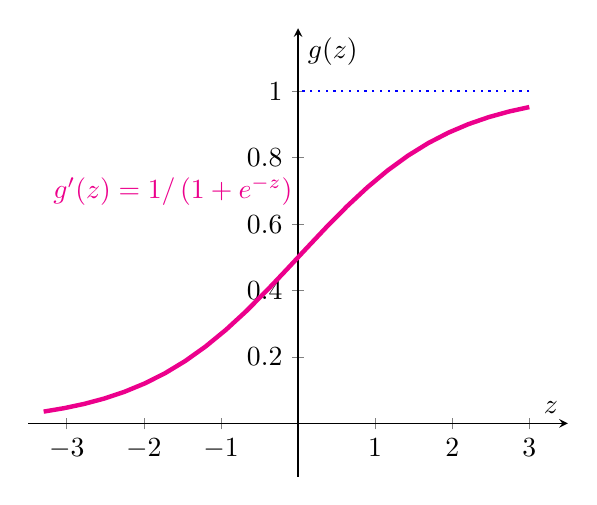
\begin{tikzpicture}
        \begin{axis}[
            xmin=-3.5, xmax=3.5,
            ymin=-.16, ymax=1.19,
            axis lines=center,
            axis on top=false,
            domain=-3.3:3,
            ylabel=$g(z)$,
            xlabel=$z$,
            ]
        
            \addplot [mark=none,draw=magenta,ultra thick] {exp(x) / (1+exp(x))};
            
            \node [right, magenta] at (axis cs: -3.3,0.7) {$g'(z) = 1/\left(1+e^{-z}\right)$};
            
            \draw [blue, dotted, thick] (axis cs:+3,+1)-- (axis cs:0,+1);
        \end{axis}
    \end{tikzpicture}
}